\begin{Schunk}
\begin{Sinput}
> library("Ham94", lib.loc = "../../../library")
\end{Sinput}
\end{Schunk}
This section uses a few utility functions that follow procedures in the test for testing hypotheses about unit roots.
First is the Newey West estimator described by [10.5.10] and [10.5.15].
\begin{Schunk}
\begin{Sinput}
> print(Newey.West)
\end{Sinput}
\begin{Soutput}
function (X, lags) 
{
    S <- 0
    T <- dim(X)[[1]]
    for (lag in lags:1) S <- S + (lags + 1 - lag)/(lags + 1) * 
        t(X[(lag + 1):T, ]) %*% X[1:(T - lag), ]
    1/T * (t(X) %*% X + S + t(S))
}
<environment: namespace:Ham94>
\end{Soutput}
\end{Schunk}
Next are the Dickey Fuller stats described in [17.4.7] and [17.4.9], with an optional correction for
serial correlation defined in [17.7.35] and [17.7.38].
\begin{Schunk}
\begin{Sinput}
> print(Dickey.Fuller)
\end{Sinput}
\begin{Soutput}
function (T, rho, sigma.rho, zeta = numeric(0)) 
{
    list(T = T, rho = rho, sigma.rho = sigma.rho, zeta = zeta, 
        rho.stat = T * (rho - 1)/(1 - sum(zeta)), t.stat = (rho - 
            1)/sigma.rho)
}
<environment: namespace:Ham94>
\end{Soutput}
\end{Schunk}
The Phillips Perron stats are defined by [17.6.8] and [17.6.12]
\begin{Schunk}
\begin{Sinput}
> print(Phillips.Perron)
\end{Sinput}
\begin{Soutput}
function (T, rho, sigma.rho, s, lambda.hat.sq, gamma0) 
{
    list(T = T, rho = rho, sigma.rho = sigma.rho, s.sq = s^2, 
        lambda.hat.sq = lambda.hat.sq, gamma0 = gamma0, rho.stat = T * 
            (rho - 1) - 1/2 * (T * sigma.rho/s)^2 * (lambda.hat.sq - 
            gamma0), t.stat = (gamma0/lambda.hat.sq)^0.5 * (rho - 
            1)/sigma.rho - 1/2 * (lambda.hat.sq - gamma0) * T * 
            sigma.rho/s/(lambda.hat.sq^0.5))
}
<environment: namespace:Ham94>
\end{Soutput}
\end{Schunk}
Finally the Wald form of an F test as defined by [8.1.32].
\begin{Schunk}
\begin{Sinput}
> print(Wald.F.Test)
\end{Sinput}
\begin{Soutput}
function (R, b, r, s2, XtX_1) 
{
    v <- R %*% b - r
    as.numeric(t(v) %*% solve(s2 * R %*% XtX_1 %*% t(R)) %*% 
        v/dim(R)[[1]])
}
<environment: namespace:Ham94>
\end{Soutput}
\end{Schunk}
\subsection{Dickey Fuller Tests for Unit Roots}
Page 489 describes the analysis of nominal
three month U.S. Treasury
yield data from
dataset gnptbill, shown below.
\begin{Schunk}
\begin{Sinput}
> data(gnptbill, package = "Ham94")
> tbill.data <- data.frame(yt = gnptbill$TBILL[-1], yt_1 = gnptbill$TBILL[-length(gnptbill$TBILL)])
\end{Sinput}
\end{Schunk}
\begin{center}
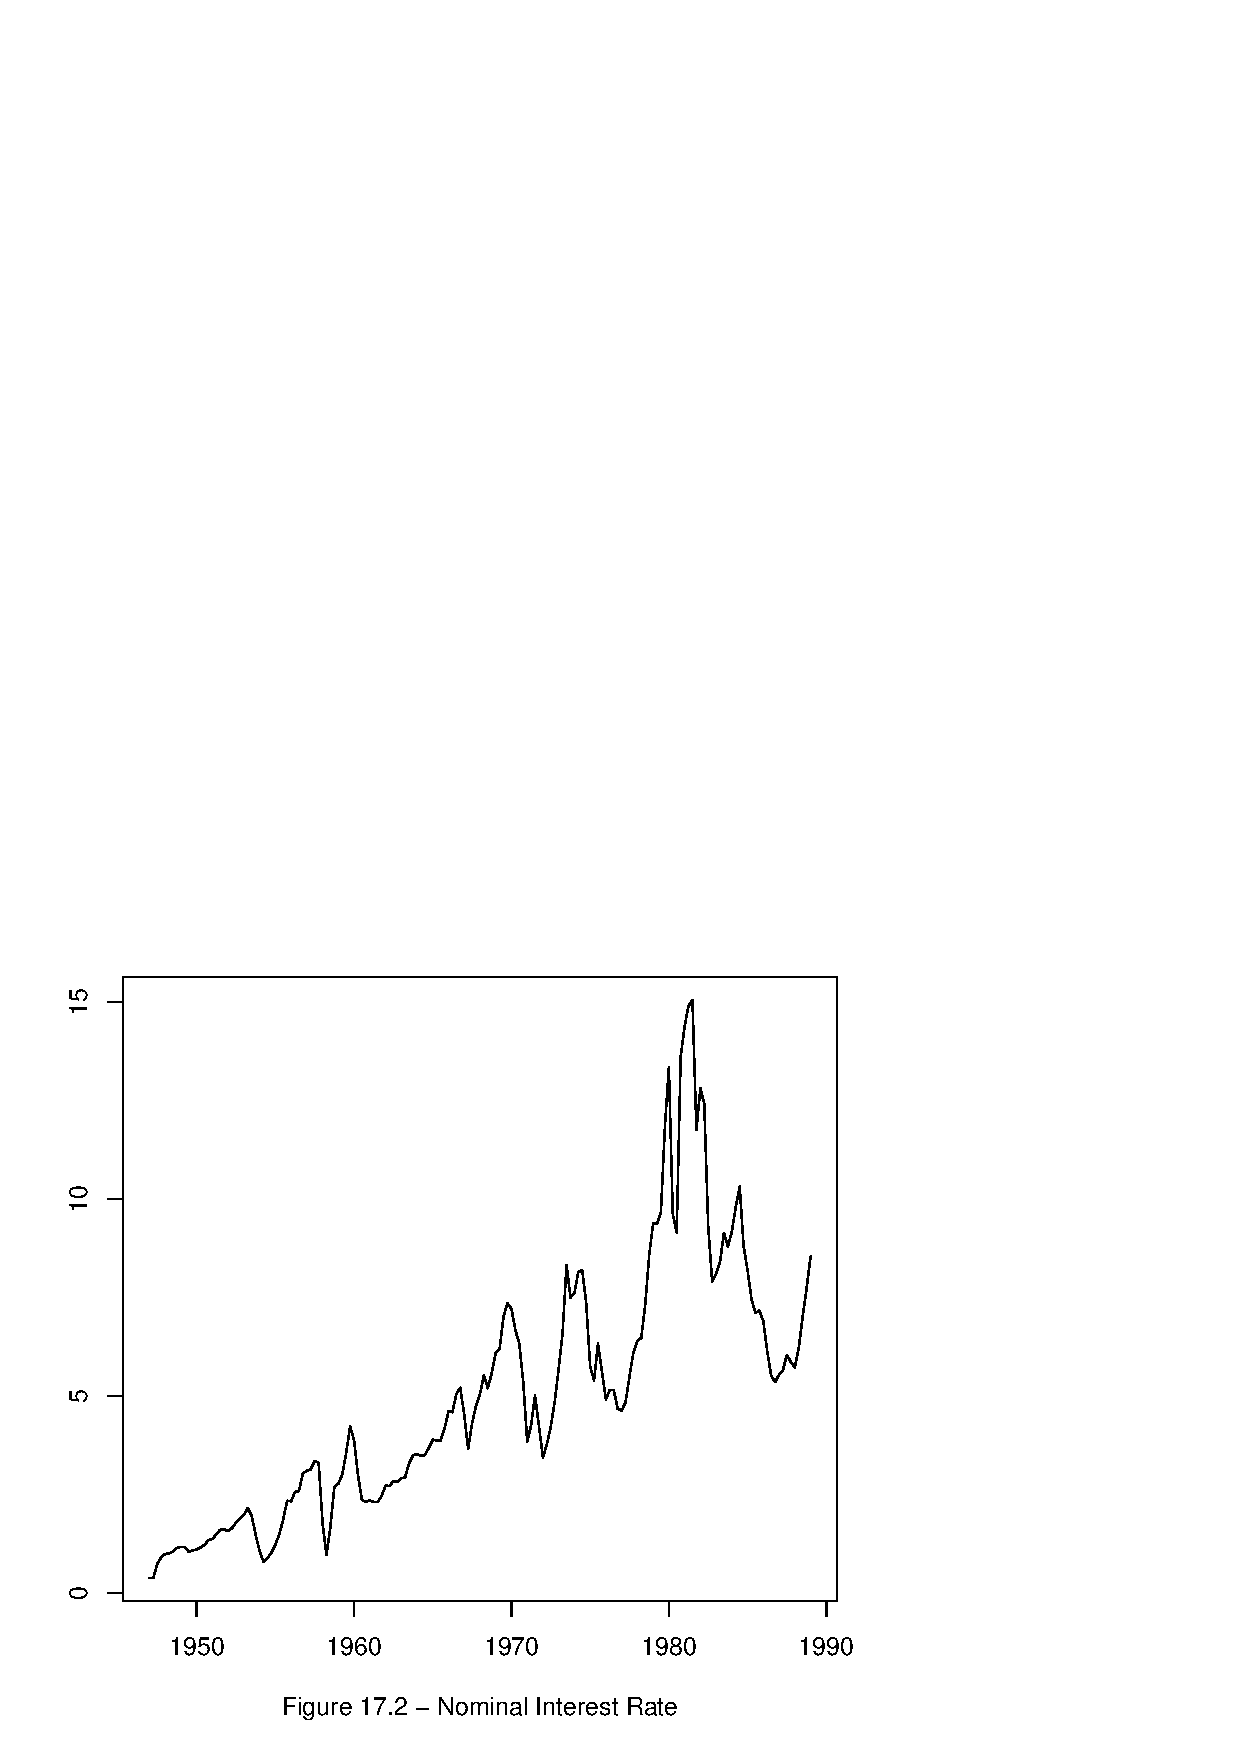
\includegraphics{p489-007}
\end{center}
The regression model is shown in [17.4.13], and the results are shown below.
\begin{Schunk}
\begin{Sinput}
> case1.lms <- summary(lm(yt ~ 0 + yt_1 + 0, tbill.data))
> case1.DF <- Dickey.Fuller(T = length(tbill.data$yt), rho = case1.lms$coefficients[["yt_1", 
+     "Estimate"]], sigma.rho = case1.lms$coefficients[["yt_1", 
+     "Std. Error"]])
> print(case1.lms$coefficients)
\end{Sinput}
\begin{Soutput}
      Estimate Std. Error  t value      Pr(>|t|)
yt_1 0.9969357 0.01059183 94.12311 1.277207e-146
\end{Soutput}
\begin{Sinput}
> print(case1.DF)
\end{Sinput}
\begin{Soutput}
$T
[1] 168

$rho
[1] 0.9969357

$sigma.rho
[1] 0.01059183

$zeta
numeric(0)

$rho.stat
[1] -0.5147943

$t.stat
[1] -0.2893034
\end{Soutput}
\end{Schunk}
A similar analysis is described on page 494 , but a constant is included in the regression model [17.4.37].
\begin{Schunk}
\begin{Sinput}
> case2.lms <- summary(lm(yt ~ 1 + yt_1, tbill.data))
> case2.DF <- Dickey.Fuller(T = length(tbill.data$yt), rho = case2.lms$coefficients[["yt_1", 
+     "Estimate"]], sigma.rho = case2.lms$coefficients[["yt_1", 
+     "Std. Error"]])
> print(case2.lms$coefficients)
\end{Sinput}
\begin{Soutput}
             Estimate Std. Error   t value      Pr(>|t|)
(Intercept) 0.2105899 0.11212302  1.878204  6.210685e-02
yt_1        0.9669104 0.01913305 50.536135 1.013453e-102
\end{Soutput}
\begin{Sinput}
> print(case2.DF)
\end{Sinput}
\begin{Soutput}
$T
[1] 168

$rho
[1] 0.9669104

$sigma.rho
[1] 0.01913305

$zeta
numeric(0)

$rho.stat
[1] -5.559061

$t.stat
[1] -1.729450
\end{Soutput}
\end{Schunk}
Example 17.5 describes how to test the joint hypothesis that the trend coefficient is 0 and the autoregressive
coefficient is 1.
\begin{Schunk}
\begin{Sinput}
> F <- Wald.F.Test(R = diag(2), b = case2.lms$coefficients[, "Estimate"], 
+     r = c(0, 1), s2 = case2.lms$sigma^2, XtX_1 = case2.lms$cov.unscaled)
> print(F)
\end{Sinput}
\begin{Soutput}
[1] 1.806307
\end{Soutput}
\end{Schunk}
\subsection{Analyzing GNP data}
A similar analysis can be conducted on log real GNP data described beginning on page 501, shown below.
\begin{Schunk}
\begin{Sinput}
> logGNP <- 100 * log(gnptbill$GNP)
> gnp.data <- data.frame(tt = seq(1, length(gnptbill$GNP) - 1), 
+     yt = logGNP[-1], yt_1 = logGNP[-length(gnptbill$GNP)])
\end{Sinput}
\end{Schunk}
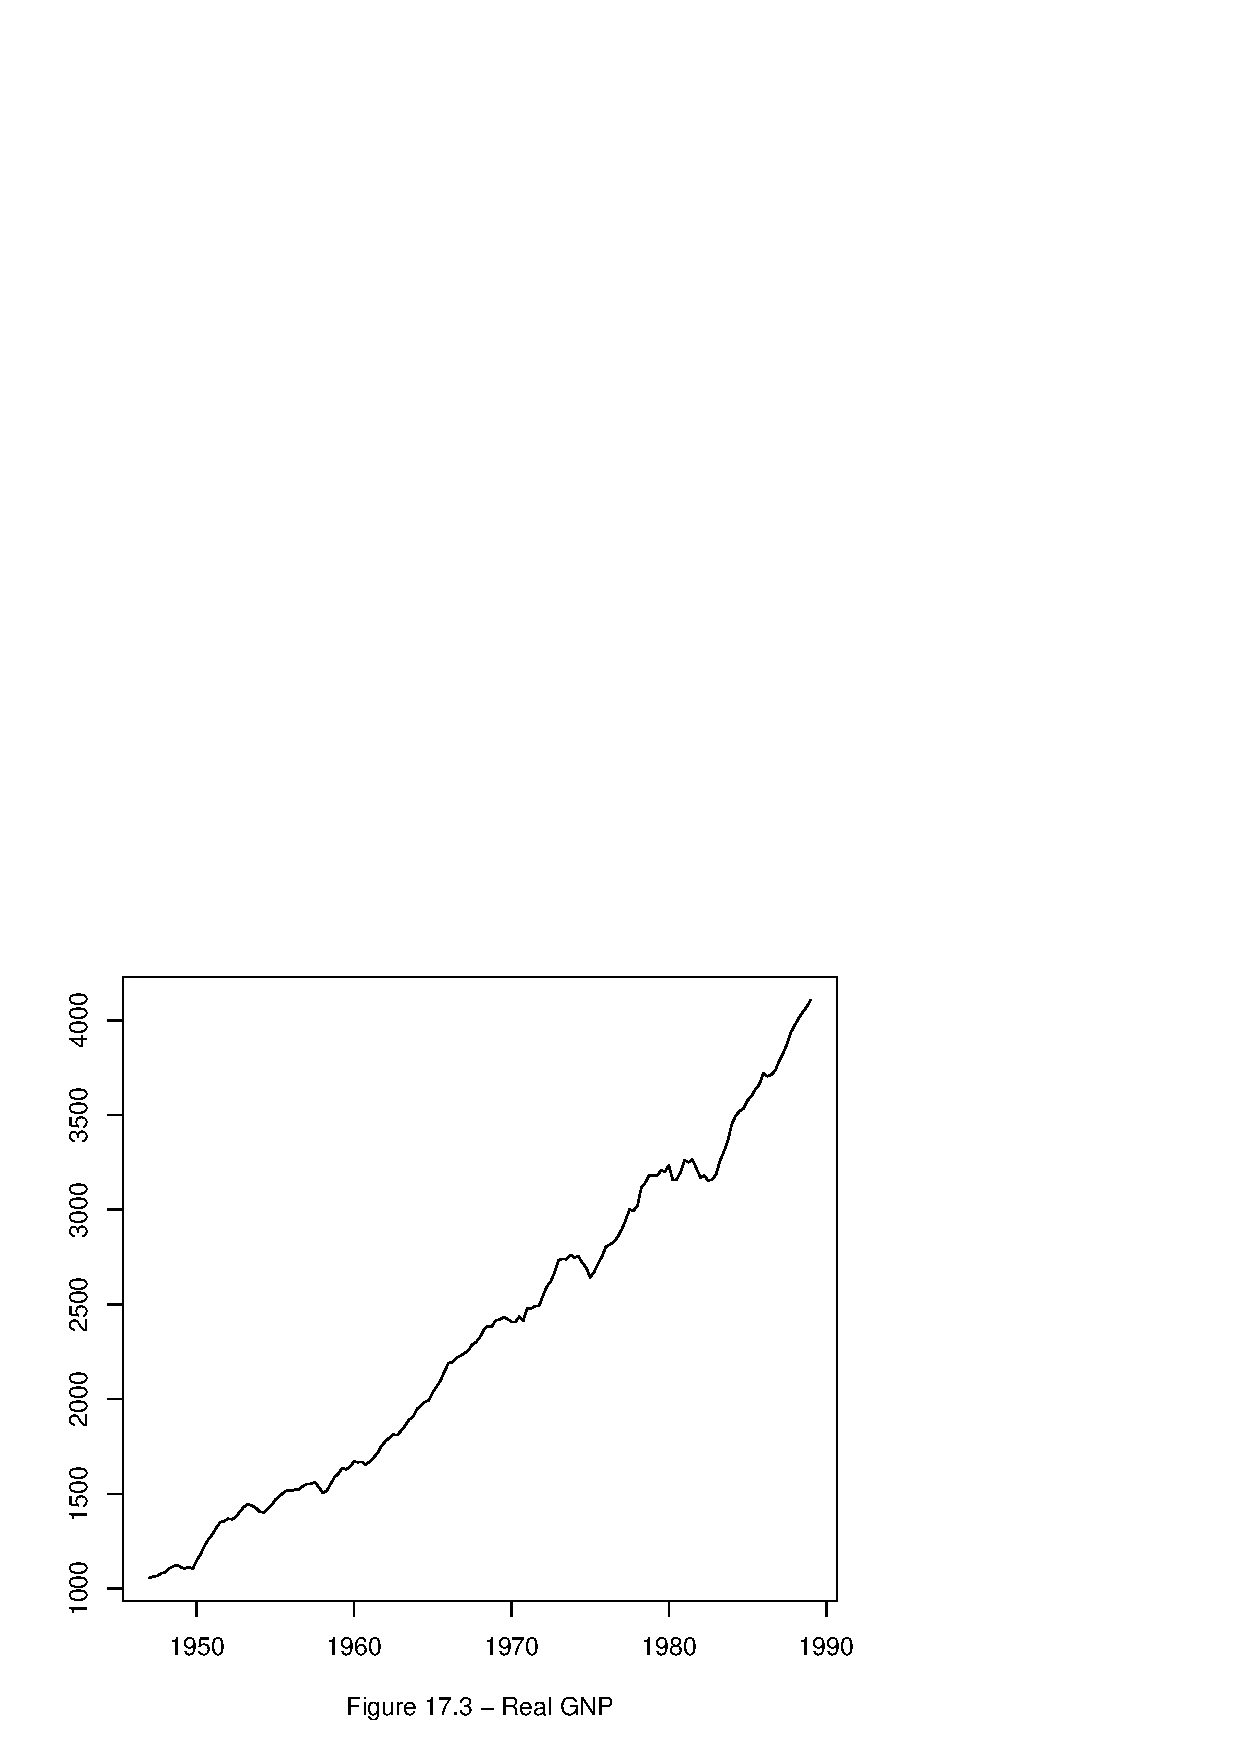
\includegraphics{p489-012}
The regression model here incorporates a time trend, based on the shape of the GDP graph
\begin{Schunk}
\begin{Sinput}
> case4.lms <- summary(lm(yt ~ 1 + yt_1 + tt, gnp.data))
> case4.DF <- Dickey.Fuller(T = length(gnp.data$yt), rho = case4.lms$coefficients[["yt_1", 
+     "Estimate"]], sigma.rho = case4.lms$coefficients[["yt_1", 
+     "Std. Error"]])
> print(case4.lms$coefficients)
\end{Sinput}
\begin{Soutput}
               Estimate  Std. Error   t value      Pr(>|t|)
(Intercept) 27.26477184 13.54992552  2.012171  4.582876e-02
yt_1         0.96252203  0.01930452 49.859941 2.076152e-101
tt           0.02753238  0.01520877  1.810296  7.206931e-02
\end{Soutput}
\begin{Sinput}
> print(case4.DF)
\end{Sinput}
\begin{Soutput}
$T
[1] 168

$rho
[1] 0.962522

$sigma.rho
[1] 0.01930452

$zeta
numeric(0)

$rho.stat
[1] -6.296298

$t.stat
[1] -1.941409
\end{Soutput}
\begin{Sinput}
> F <- Wald.F.Test(R = cbind(rep(0, 2), diag(2)), b = case4.lms$coefficients[, 
+     "Estimate"], r = c(1, 0), s2 = case4.lms$sigma^2, XtX_1 = case4.lms$cov.unscaled)
> print(F)
\end{Sinput}
\begin{Soutput}
[1] 2.442251
\end{Soutput}
\end{Schunk}

\subsection{Using Phillips Perron Tests}
Examples 17.6 and 17.7 reanalyze the case 2 and case 4 regressions above using the Phillips Perron tests
as shown on pages 511-513.
\begin{Schunk}
\begin{Sinput}
> case2.PP <- Phillips.Perron(T = length(case2.lms$residuals), 
+     rho = case2.lms$coefficients[["yt_1", "Estimate"]], sigma.rho = case2.lms$coefficients[["yt_1", 
+         "Std. Error"]], s = case2.lms$sigma, lambda.hat.sq = as.numeric(Newey.West(case2.lms$residuals %o% 
+         1, 4)), gamma0 = mean(case2.lms$residuals^2))
> print(case2.lms$coefficients)
\end{Sinput}
\begin{Soutput}
             Estimate Std. Error   t value      Pr(>|t|)
(Intercept) 0.2105899 0.11212302  1.878204  6.210685e-02
yt_1        0.9669104 0.01913305 50.536135 1.013453e-102
\end{Soutput}
\begin{Sinput}
> print(case2.PP)
\end{Sinput}
\begin{Soutput}
$T
[1] 168

$rho
[1] 0.9669104

$sigma.rho
[1] 0.01913305

$s.sq
[1] 0.6375998

$lambda.hat.sq
[1] 0.6880069

$gamma0
[1] 0.6300093

$rho.stat
[1] -6.028975

$t.stat
[1] -1.795686
\end{Soutput}
\begin{Sinput}
> case4.PP <- Phillips.Perron(T = length(case4.lms$residuals), 
+     rho = case4.lms$coefficients[["yt_1", "Estimate"]], sigma.rho = case4.lms$coefficients[["yt_1", 
+         "Std. Error"]], s = case4.lms$sigma, lambda.hat.sq = as.numeric(Newey.West(case4.lms$residuals %o% 
+         1, 4)), gamma0 = mean(case4.lms$residuals^2))
> print(case4.lms$coefficients)
\end{Sinput}
\begin{Soutput}
               Estimate  Std. Error   t value      Pr(>|t|)
(Intercept) 27.26477184 13.54992552  2.012171  4.582876e-02
yt_1         0.96252203  0.01930452 49.859941 2.076152e-101
tt           0.02753238  0.01520877  1.810296  7.206931e-02
\end{Soutput}
\begin{Sinput}
> print(case4.PP)
\end{Sinput}
\begin{Soutput}
$T
[1] 168

$rho
[1] 0.962522

$sigma.rho
[1] 0.01930452

$s.sq
[1] 1.156270

$lambda.hat.sq
[1] 2.117173

$gamma0
[1] 1.135623

$rho.stat
[1] -10.76066

$t.stat
[1] -2.439143
\end{Soutput}
\end{Schunk}
\subsection{Augmented Dickey Fuller Tests}
Example 17.8 illustrates incorporates the use of lagged regressors to (putatively) eliminate serial
correlation in the residuals.  The function "embed" is useful for creating lagged regressors.
\begin{Schunk}
\begin{Sinput}
> tbill.data <- list(it = gnptbill$TBILL[-1:-5], delta.it_ = embed(diff(gnptbill$TBILL[-length(gnptbill$TBILL)]), 
+     4), it_1 = gnptbill$TBILL[c(-1:-4, -(length(gnptbill$TBILL):length(gnptbill$TBILL)))])
> tbill.lms <- summary(lm(it ~ delta.it_ + 1 + it_1, tbill.data))
> tbill.adf <- Dickey.Fuller(T = length(gnptbill$TBILL) - 5, rho = tbill.lms$coefficients[["it_1", 
+     "Estimate"]], sigma.rho = tbill.lms$coefficients[["it_1", 
+     "Std. Error"]], zeta = tbill.lms$coefficients[paste("delta.it", 
+     1:4, sep = "_"), "Estimate"])
> print(tbill.lms$coefficients)
\end{Sinput}
\begin{Soutput}
              Estimate Std. Error   t value      Pr(>|t|)
(Intercept)  0.1954328 0.10863764  1.798942  7.393646e-02
delta.it_1   0.3346654 0.07882340  4.245762  3.705074e-05
delta.it_2  -0.3879736 0.08082096 -4.800408  3.643800e-06
delta.it_3   0.2761332 0.07998276  3.452409  7.130684e-04
delta.it_4  -0.1067090 0.07944645 -1.343156  1.811475e-01
it_1         0.9690445 0.01860387 52.088332 2.094220e-101
\end{Soutput}
\begin{Sinput}
> print(tbill.adf)
\end{Sinput}
\begin{Soutput}
$T
[1] 164

$rho
[1] 0.9690445

$sigma.rho
[1] 0.01860387

$zeta
delta.it_1 delta.it_2 delta.it_3 delta.it_4 
 0.3346654 -0.3879736  0.2761332 -0.1067090 

$rho.stat
[1] -5.74363

$t.stat
[1] -1.663928
\end{Soutput}
\end{Schunk}
The next test checks whether or not the farthest lag is different from zero, i.e. whether or not the right number
of lags are included in the equation.
\begin{Schunk}
\begin{Sinput}
> print(tbill.lms$coefficients[["delta.it_4", "t value"]])
\end{Sinput}
\begin{Soutput}
[1] -1.343156
\end{Soutput}
\end{Schunk}
Example 17.9 performs a similar analysis for the GNP data. 
\begin{Schunk}
\begin{Sinput}
> gnp.data <- list(yt = logGNP[-1:-5], delta.yt_ = embed(diff(logGNP[-length(logGNP)]), 
+     4), yt_1 = logGNP[c(-1:-4, -(length(logGNP):length(logGNP)))], 
+     t = 6:length(logGNP))
> gnp.lms <- summary(lm(yt ~ delta.yt_ + 1 + yt_1 + t, gnp.data))
> gnp.adf <- Dickey.Fuller(T = length(logGNP) - 5, rho = gnp.lms$coefficients[["yt_1", 
+     "Estimate"]], sigma.rho = gnp.lms$coefficients[["yt_1", "Std. Error"]], 
+     zeta = gnp.lms$coefficients[paste("delta.yt", 1:4, sep = "_"), 
+         "Estimate"])
> F <- Wald.F.Test(R = cbind(rep(0, 2) %o% rep(0, 5), diag(2)), 
+     b = gnp.lms$coefficients[, "Estimate"], r = c(1, 0), s2 = gnp.lms$sigma^2, 
+     XtX_1 = gnp.lms$cov.unscaled)
> print(gnp.lms$coefficients)
\end{Sinput}
\begin{Soutput}
               Estimate  Std. Error    t value     Pr(>|t|)
(Intercept) 35.91807717 13.57200191  2.6464834 8.961726e-03
delta.yt_1   0.32908487  0.07769385  4.2356619 3.869829e-05
delta.yt_2   0.20856825  0.08128118  2.5660092 1.122316e-02
delta.yt_3  -0.08424648  0.08182895 -1.0295437 3.048077e-01
delta.yt_4  -0.07453301  0.07879621 -0.9458959 3.456552e-01
yt_1         0.94969015  0.01938565 48.9893326 4.883651e-97
t            0.03783123  0.01521561  2.4863440 1.395295e-02
\end{Soutput}
\begin{Sinput}
> print(gnp.adf)
\end{Sinput}
\begin{Soutput}
$T
[1] 164

$rho
[1] 0.9496901

$sigma.rho
[1] 0.01938565

$zeta
 delta.yt_1  delta.yt_2  delta.yt_3  delta.yt_4 
 0.32908487  0.20856825 -0.08424648 -0.07453301 

$rho.stat
[1] -13.28363

$t.stat
[1] -2.595211
\end{Soutput}
\begin{Sinput}
> print(F)
\end{Sinput}
\begin{Soutput}
[1] 3.743228
\end{Soutput}
\end{Schunk}
\subsection{Example 17.10 - Bayesian Test of Autoregressive Coefficient}
Page 532 describes a test on the autoregressive coefficient that weights prior probabilities.
\begin{Schunk}
\begin{Sinput}
> t.value <- (1 - gnp.lms$coefficients[["yt_1", "Estimate"]])/gnp.lms$coefficients[["yt_1", 
+     "Std. Error"]]
> print(t.value)
\end{Sinput}
\begin{Soutput}
[1] 2.595211
\end{Soutput}
\begin{Sinput}
> print((1 - pt(t.value, 164))/2)
\end{Sinput}
\begin{Soutput}
[1] 0.002577594
\end{Soutput}
\end{Schunk}
\subsection{Determining Lag Length}
Page 530 describes an iterative process to determine the correct lag length.  This is easily expressed
in terms of the structures used above.
\begin{Schunk}
\begin{Sinput}
> for (lag in 10:1) {
+     gnp.lm <- lm(yt ~ delta.yt_ + 1 + yt_1 + t, list(yt = logGNP[-1:-(lag + 
+         1)], delta.yt_ = embed(diff(logGNP[-length(logGNP)]), 
+         lag), yt_1 = logGNP[c(-1:-lag, -(length(logGNP):length(logGNP)))], 
+         t = (lag + 2):length(logGNP)))
+     if (summary(gnp.lm)$coefficients[[paste("delta.yt", lag, 
+         sep = "_"), "Pr(>|t|)"]] < 0.05) 
+         break
+ }
> print(lag)
\end{Sinput}
\begin{Soutput}
[1] 2
\end{Soutput}
\end{Schunk}
\subsection{R Facilities for Testing Unit Roots}
TBD

